\documentclass{article}
\usepackage{graphicx}
\usepackage[margin=1.5cm]{geometry}
\usepackage{amsmath}

\begin{document}

\title{Thursday Reading Assessment: ADC and DAC (Chapter 12 + Lab)}
\author{Prof. Jordan C. Hanson}

\maketitle

\begin{figure}[ht]
\centering
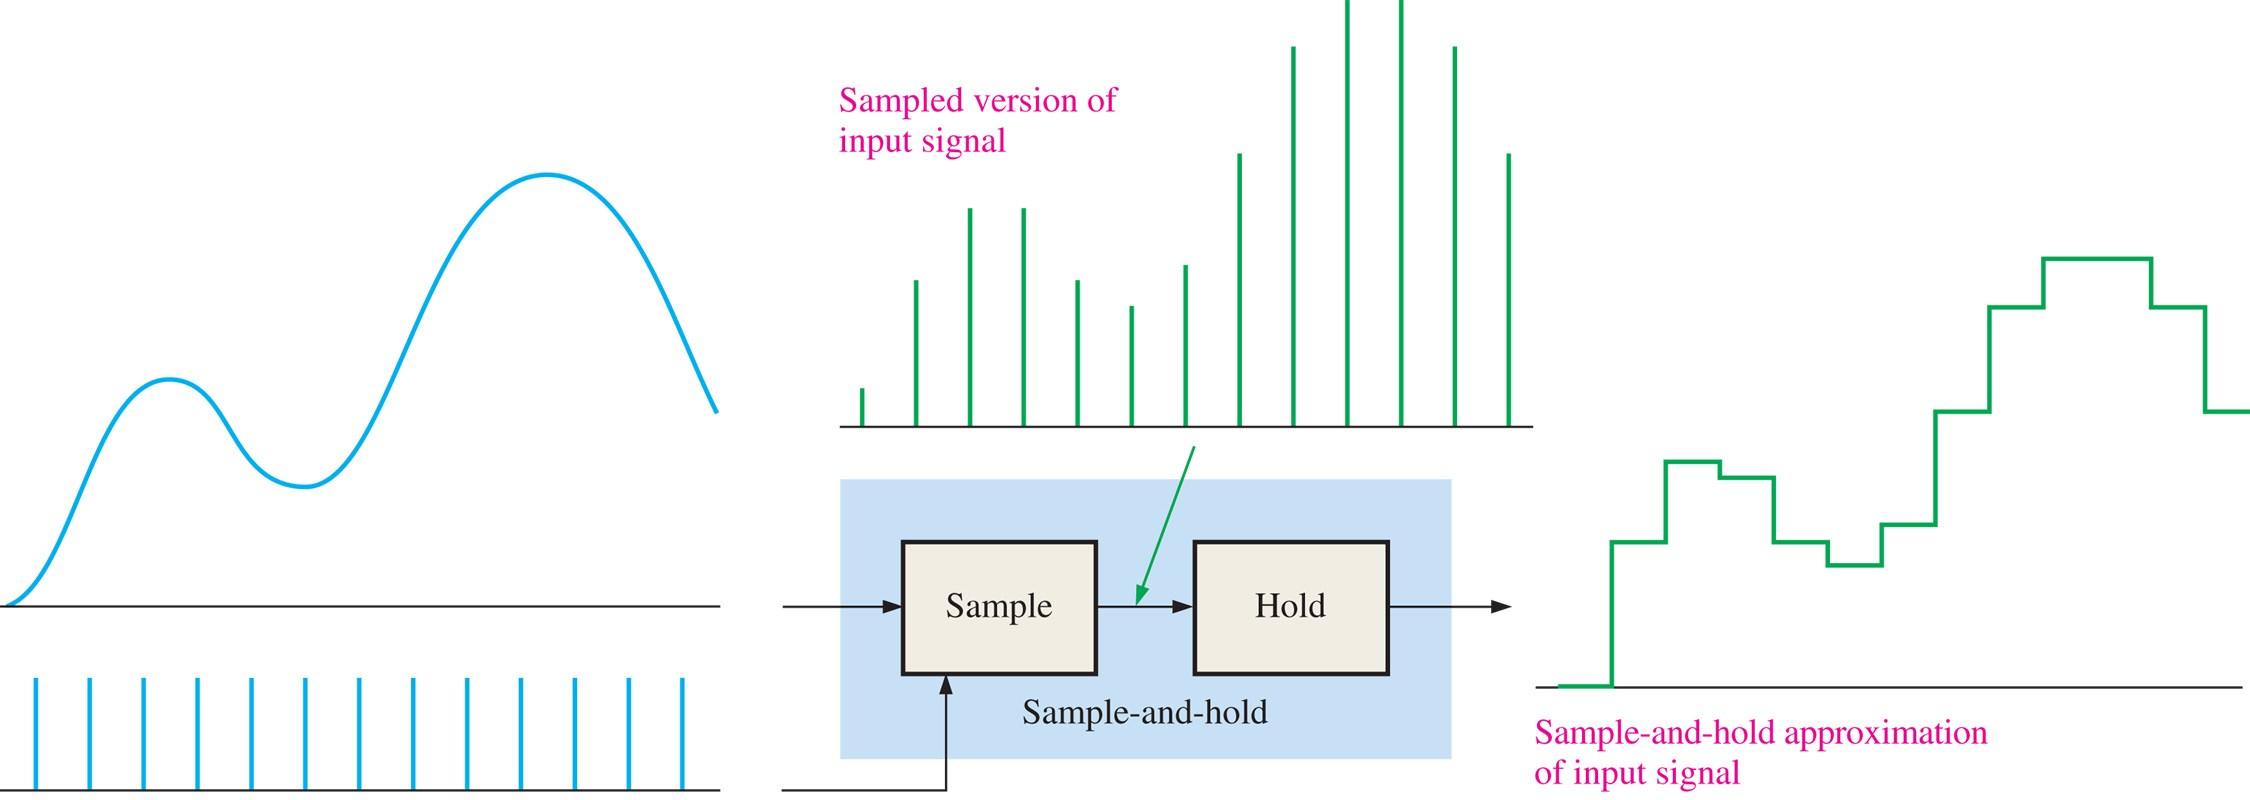
\includegraphics[width=0.55\textwidth]{figures/adc_1.jpg}
\caption{\label{fig:1} Simple picture of the sample-and-hold step in analog-to-digital conversion.}
\end{figure}

\section{Analog-to-Digital Conversion}

\begin{enumerate}
\item \textbf{Analog-to-digital conversion} (ADC) is a 2-step process by which analog signals are converted to digital data in digital circuits.  The first step is depicted in Fig. \ref{fig:1} (top left, top right).  In a \textbf{sample-and-hold} operation, the continuous signal is mixed with \textit{sample pulses} emitted at rate equal to the sampling frequency.  (Fig. \ref{fig:1} (top left)).  The mixed sample pulses then cause a latch to \textit{hold} the voltage value for the duration of the sample, $\Delta t = f_s^{-1}$ (Fig. \ref{fig:1} (top right)).  (a) If $\Delta t$ is 1 $\mu$s, what is the sampling frequency?  (b) What is the Nyquist frequency? \\ \vspace{2cm}
\item In the next stage of ADC, the sample-and-hold output is \textit{digitized}.  Assume the space between maximum voltage, $V_{\rm CC}$, and 0V, is quantized with $N$ bits.  (a) If $V_{\rm CC} = 5.0$ V, and $N = 3$ bits, what is the voltage resolution? (b) If $V_{\rm CC} = 12.0$ V, and $N = 12$ bits, what is the voltage resolution? (c) If we need at least 10 mV precision for $V_{\rm CC} = 5.0$ V, what is the minimum number of ADC bits?
\end{enumerate}

\begin{figure}[ht]
\centering
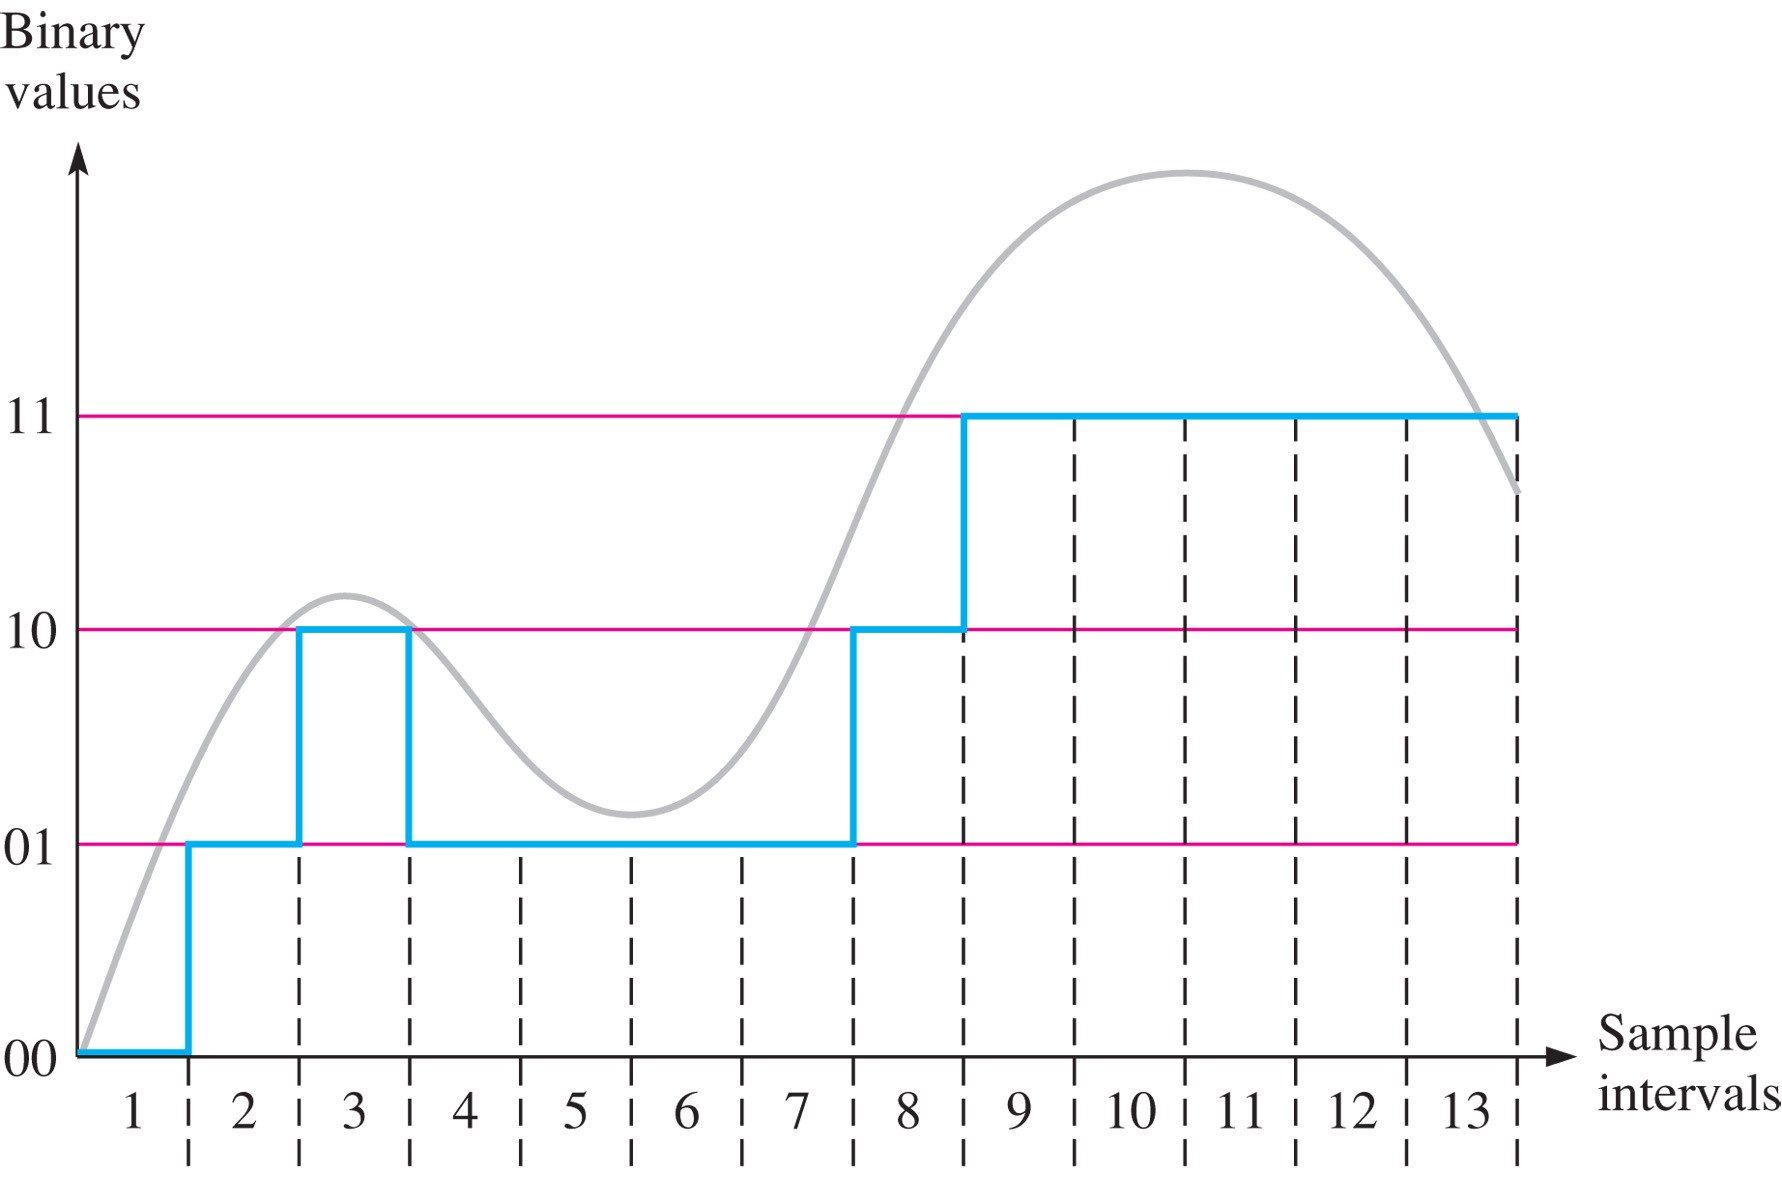
\includegraphics[width=0.4\textwidth]{figures/adc_3.jpg} \hspace{0.2cm}
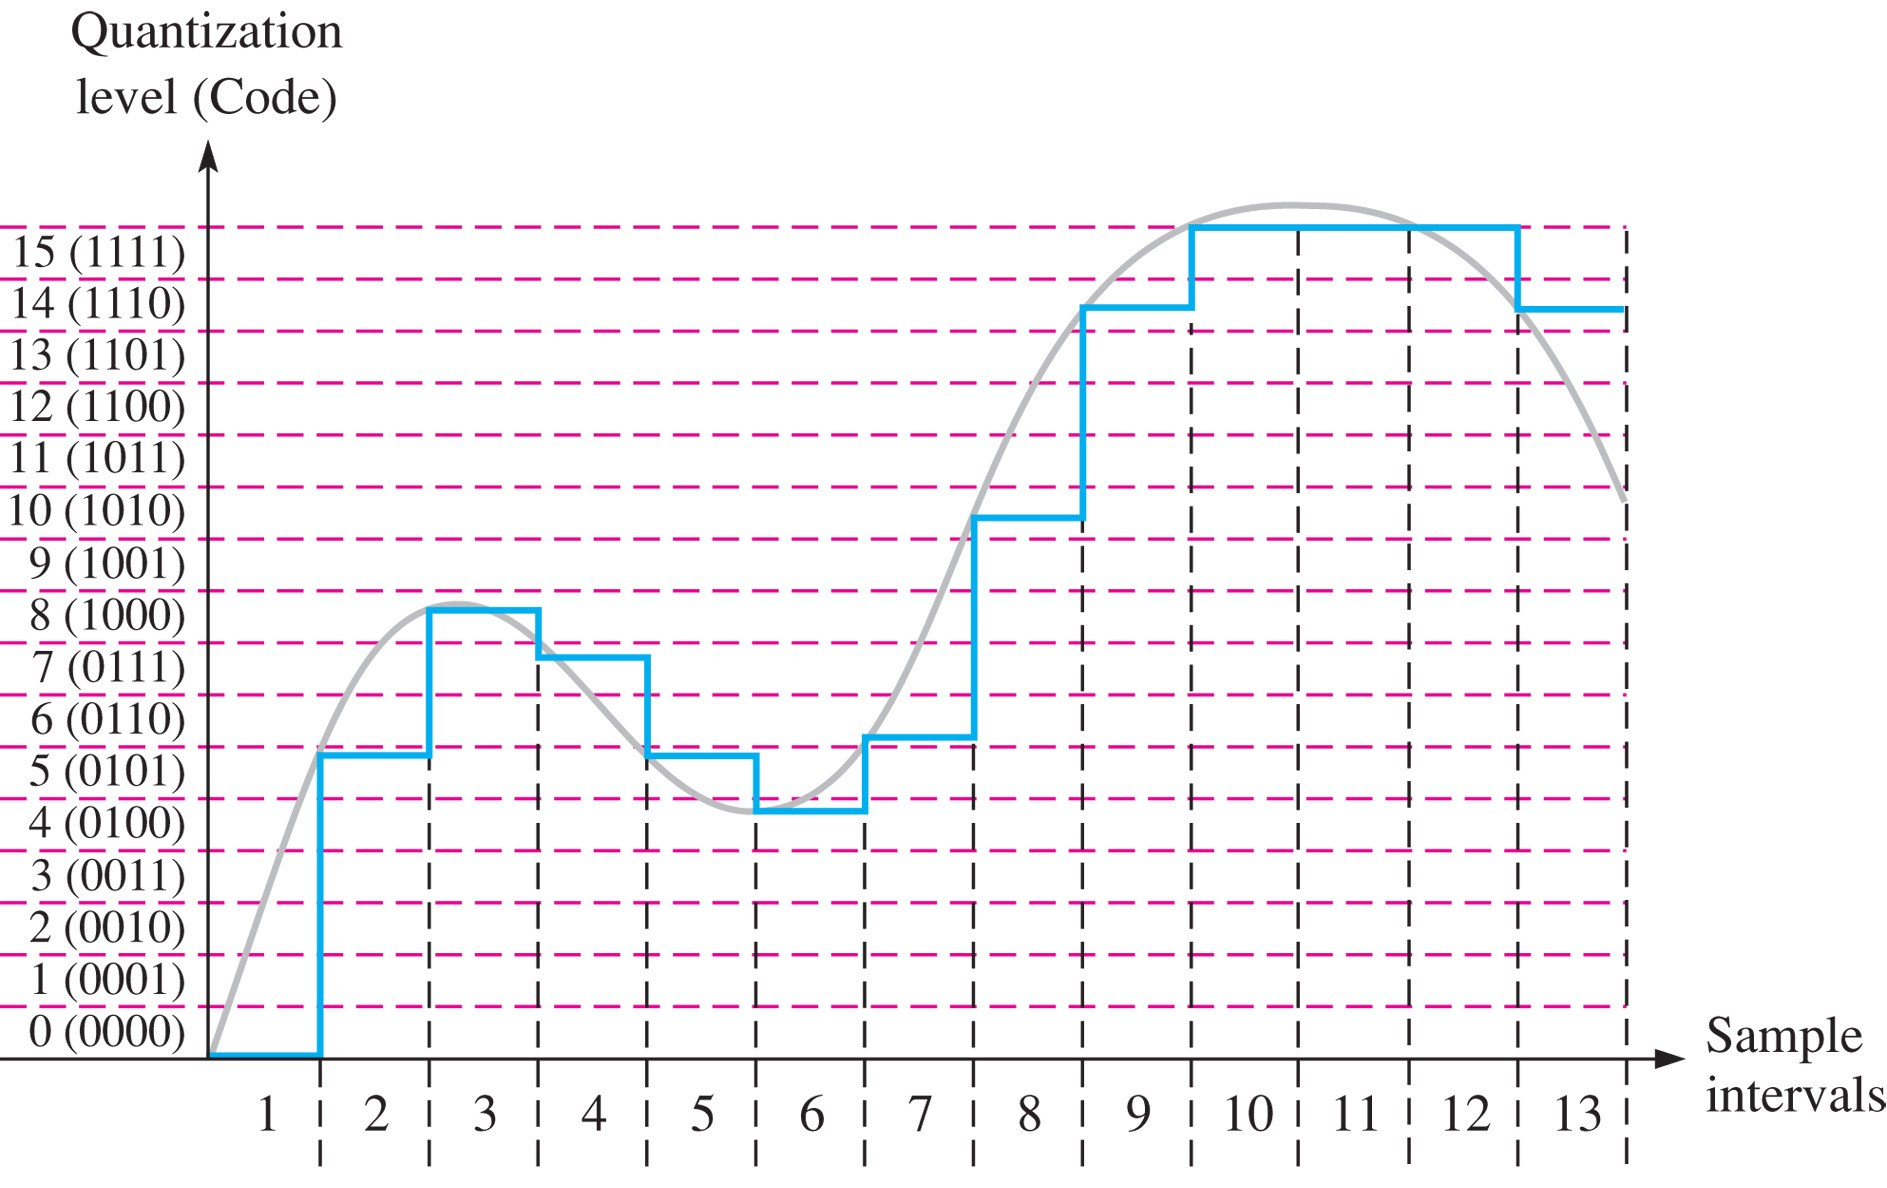
\includegraphics[width=0.4\textwidth]{figures/adc_4.jpg}
\caption{\label{fig:2} (Left) 2-bit ADC precision. (Right) 4-bit ADC precision.}
\end{figure}

\clearpage

\begin{figure}[ht]
\centering
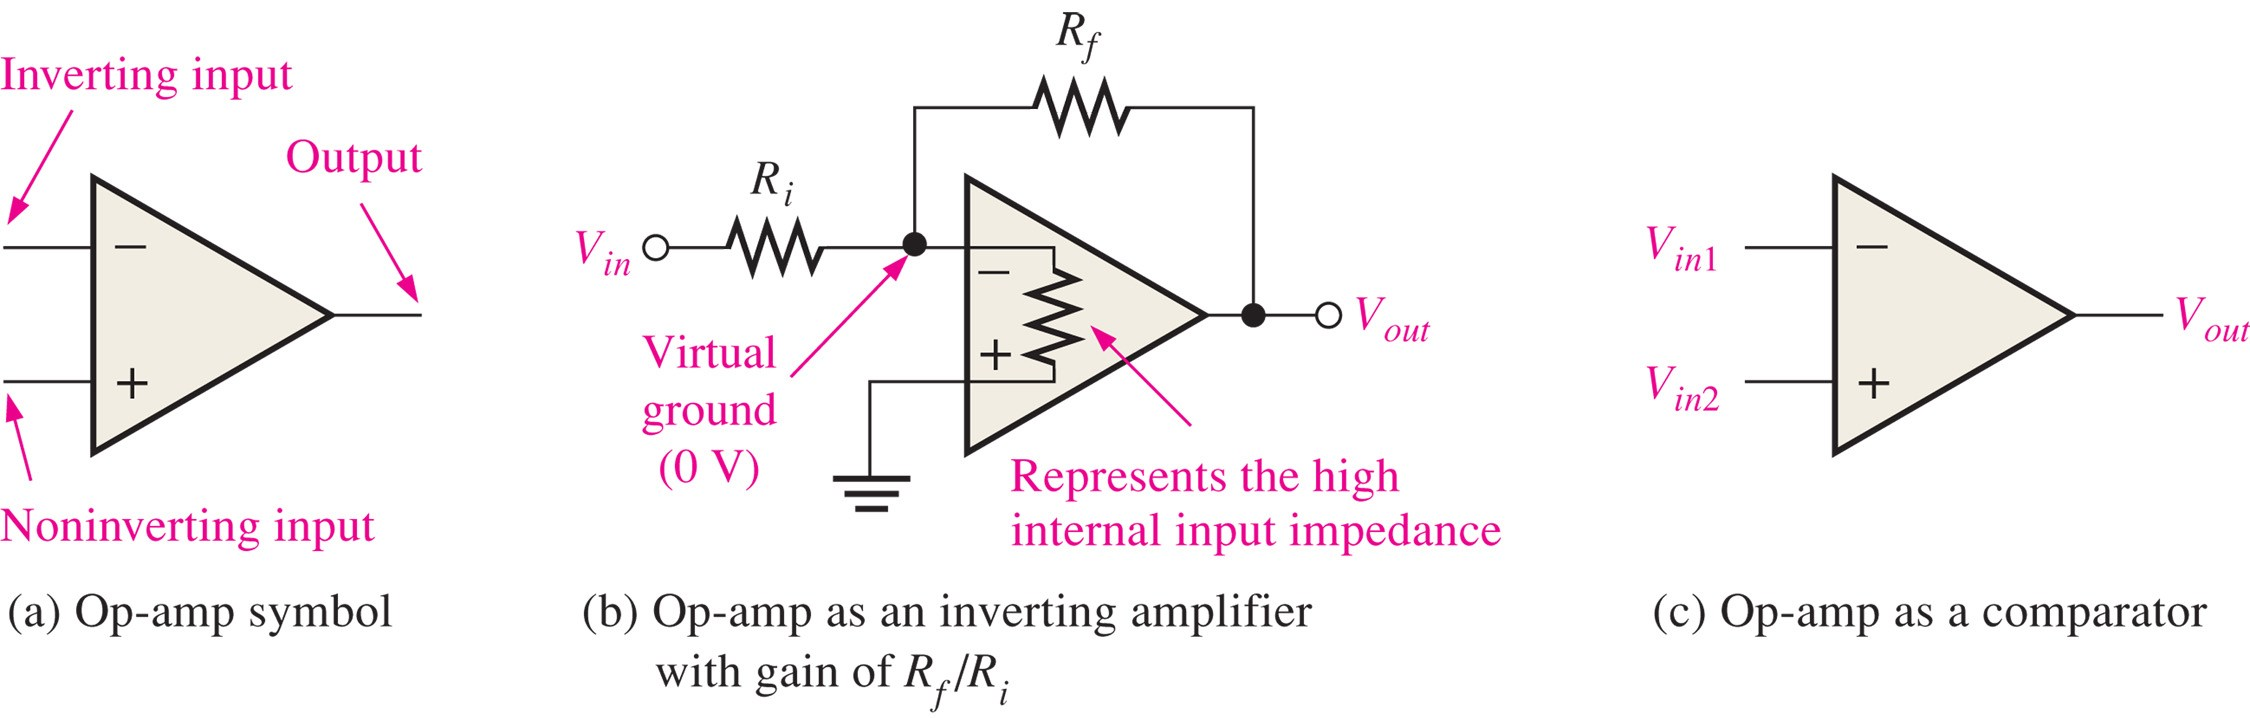
\includegraphics[width=0.65\textwidth]{figures/adc_5.jpg} \\ \vspace{1cm}
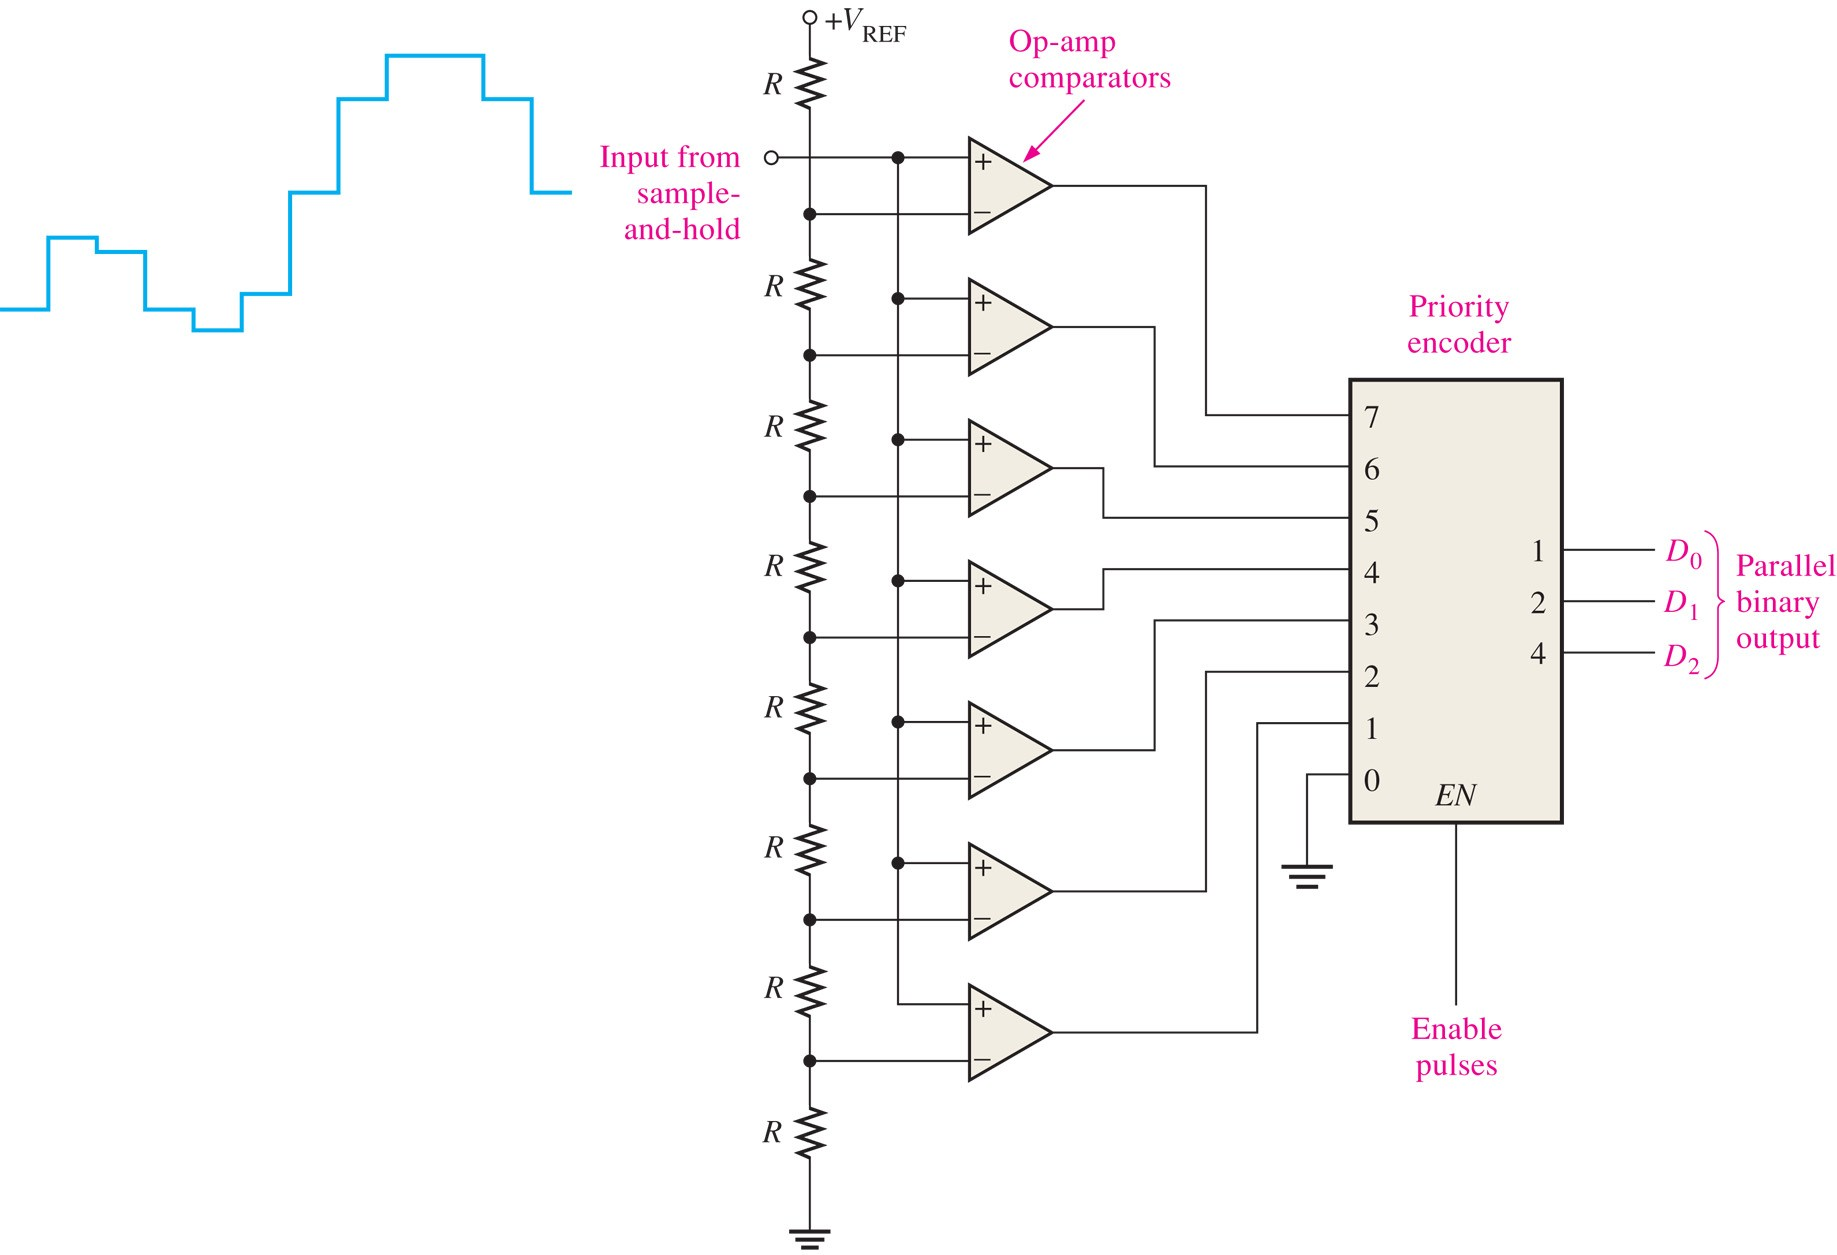
\includegraphics[width=0.65\textwidth]{figures/adc_6.jpg}
\caption{\label{fig:2} (Top) Op-amp characteristics. (Bottom) 3-bit flash ADC schematic.}
\end{figure}

\end{document}
